\subsection{Comparing the different regularizations}  \label{sec:num_regularization}

As noted in section~\ref{sec:regularization}, the quasi-static
force-free model requires regularization that invokes either a
fictitious drag coefficient $\epsilon$ or an artificial viscosity
$\nu.$ Since they enter directly into the force-balance equation that
would otherwise constrain the magnetic field to be force-free, we
anticipate their presence will modify the quasi-static dynamics but
the effect will diminish as $\epsilon$ or $\nu$ gets smaller. This is
a convergence issue related to modeling $\mathbf{B}(\mathbf{x},t)$ as a function of
decreasing $\epsilon$ and $\nu.$ It is important to note that with
smaller $\epsilon$ or $\nu,$ the regularization becomes weaker so the
numerical matrix inversion for the implicit solve of the quasi-static
model becomes more difficult computationally. So a practically useful
regularization scheme should produce good convergence in
$\mathbf{B}(\mathbf{x},t)$ solution for modestly small $\epsilon$ or
$\nu.$ For this convergence check, we will gauge the quality of the
solution for $\mathbf{B}$ through two quantities.  The first is the
vertical position of the magnetic axis $Z_a$ as a function of time
during a VDE.  The second is the total toroidal plasma current in the
chamber, $I_p(t),$ as a function of time during a VDE. Next we first
explain the set up of the test case, and then show how $Z_a(t)$ and
$I_p(t)$ scale with $\epsilon$ and $\nu.$

\begin{comment}
\subsection{Lundquist number $S = 2.7* 10^7$}
\end{comment}

We consider a 5-layer configuration for the resistivity as shown in
Figure~\ref{fig:5layer} with the following resistivity values:
\begin{itemize}
    \item $\eta = \SI{9.66e-6}{\ohm\meter}$ in the plasma chamber
      corresponding to values 1 and 2 for the levelset function in
      Figure~\ref{fig:5layer};
%    \item $\eta = 10^{-5}$ in the outer area of the plasma chamber located between the separatrix and the wall. This region corresponds to a value of 2 for the levelset function in Figure~\ref{fig:4layer}.     
    \item $\eta = \SI{4.4e-2}{\ohm\meter}$ in the blanket module
      corresponding to a value of 0 for the levelset function in
      Figure~\ref{fig:5layer};
    \item $\eta = \SI{1.30288e-6}{\ohm\meter}$ in the vacuum vessel
      corresponding to a value of -1 for the levelset function in
      Figure~\ref{fig:5layer};
    \item $\eta = \SI{1.30288e-3}{\ohm\meter}$ in the region
      outside the wall corresponding to a value of -2 for the levelset
      function in Figure~\ref{fig:5layer}.
\end{itemize}
and compare the results of the quasi-static models with fictitious
drag term~\eqref{eq:drag-regularize} and with fictitious viscous
term~\eqref{eq:viscous-regularize} using different viscosity and drag
coefficients. We plot the evolution in time of the $z$ coordinate of the
magnetic axis and the current intensity in
Figures~\ref{fig:z_magneticaxis_15_15eV_time}
and~\ref{fig:current_time}. Note that after normalization of
Equation~\eqref{eq:viscous-regularize}, $\mu_0 \nu$ gets replaced by
the viscosity coefficient ${1}/{Re}$.

\begin{figure}[!h]
\centering
\begin{subfigure}[b]{0.47\textwidth} 
\centering
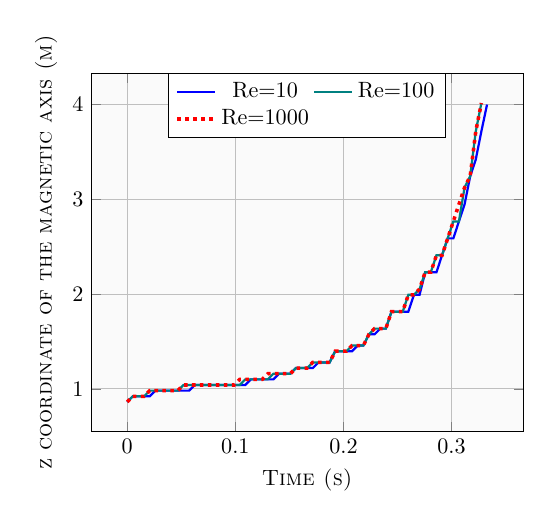
\begin{tikzpicture}[scale=0.8,>=latex]
\begin{axis}[xlabel=\textsc{{Time (s)}}, ylabel=\textsc{{z coordinate of the magnetic axis (m)}}, ymajorgrids, xmajorgrids, axis background/.style={fill=gray!4}, legend style={legend columns=2,at={(0.5,1.0)},anchor=north}]
\addplot+[color=blue,line width=1pt,mark=none] coordinates {(0, 0.86275)	(0.0052, 0.92225)	(0.0104, 0.92225)	(0.0156, 0.92225)	(0.0208, 0.92225)	(0.026, 0.98175)	(0.0312, 0.98175)	(0.0364, 0.98175)	(0.0416, 0.98175)	(0.0468, 0.98175)	(0.052, 0.98175)	(0.0572, 0.98175)	(0.0624, 1.04125)	(0.0676, 1.04125)	(0.0728, 1.04125)	(0.078, 1.04125)	(0.0832, 1.04125)	(0.0884, 1.04125)	(0.0936, 1.04125)	(0.0988, 1.04125)	(0.104, 1.04125)	(0.1092, 1.04125)	(0.1144, 1.10075)	(0.1196, 1.10075)	(0.1248, 1.10075)	(0.13, 1.10075)	         (0.1352, 1.10075)	(0.1404, 1.16025)	(0.1456, 1.16025)	(0.1508, 1.16025)	(0.156, 1.21975)	(0.1612, 1.21975)	(0.1664, 1.21975)	(0.1716, 1.21975)	(0.1768, 1.27925)	(0.182, 1.27925)	(0.1872, 1.27925)	(0.1924, 1.39825)	(0.1976, 1.39825)	(0.2028, 1.39825)	(0.208, 1.39825)	(0.2132, 1.45775)	(0.2184, 1.45775)	(0.2236, 1.57675)	(0.2288, 1.57675)   (0.234, 1.63625)	(0.2392, 1.63625)	(0.2444, 1.81475)	(0.2496, 1.81475)	(0.2548, 1.81475)	(0.26, 1.81475)   (0.2652, 1.99325)     (0.2704, 1.99325)     (0.2756, 2.23125)     (0.2808, 2.23125)     (0.286, 2.23125)       (0.2912, 2.40975)   (0.2964, 2.58825)     (0.3016, 2.58825)     (0.3068, 2.76675)     (0.3120, 2.94525)     (0.3172, 3.24275)     (0.3224, 3.42125)   (0.3276, 3.71875)   (0.3328, 4)};
\addplot+[color=teal,line width=1pt,mark=none] coordinates {(0, 0.86275)	(0.0052, 0.92225)	(0.0104, 0.92225)	(0.0156, 0.92225)	(0.0208, 0.98175)	(0.026, 0.98175)	(0.0312, 0.98175)	(0.0364, 0.98175)	(0.0416, 0.98175)	(0.0468, 0.98175)	(0.052, 1.04125)	(0.0572, 1.04125)	(0.0624, 1.04125)	(0.0676, 1.04125)	(0.0728, 1.04125)	(0.078, 1.04125)	(0.0832, 1.04125)	(0.0884, 1.04125)	(0.0936, 1.04125)	(0.0988, 1.04125)	(0.104, 1.04125)	(0.1092, 1.10075)	(0.1144, 1.10075)	(0.1196, 1.10075)	(0.1248, 1.10075)	(0.13, 1.10075)	         (0.1352, 1.16025)	(0.1404, 1.16025)	(0.1456, 1.16025)	(0.1508, 1.16025)	(0.156, 1.21975)	(0.1612, 1.21975)	(0.1664, 1.21975)	(0.1716, 1.27925)	(0.1768, 1.27925)	(0.182, 1.27925)	(0.1872, 1.27925)	(0.1924, 1.39825)	(0.1976, 1.39825)	(0.2028, 1.39825)	(0.208, 1.45775)	(0.2132, 1.45775)	(0.2184, 1.45775)	(0.2236, 1.57675)	(0.2288, 1.63625)   (0.234, 1.63625)	(0.2392, 1.63625)	(0.2444, 1.81475)	(0.2496, 1.81475)	(0.2548, 1.81475)	(0.26, 1.99325)   (0.2652, 1.99325)     (0.2704, 2.05275)     (0.2756, 2.23125)     (0.2808, 2.23125)     (0.286, 2.40975)       (0.2912, 2.40975)   (0.2964, 2.58825)     (0.3016, 2.76675)     (0.3068, 2.76675)     (0.3120, 3.12375)     (0.3172, 3.24275)     (0.3224, 3.71875)   (0.3276, 4.01625)};
\addplot+[color=red,line width=1pt,mark=none,ultra thick,dotted] coordinates {(0, 0.86275)	   (0.0052, 0.92225)	(0.0104, 0.92225)	(0.0156, 0.92225)	(0.0208, 0.98175)	(0.026, 0.98175)	(0.0312, 0.98175)	(0.0364, 0.98175)	(0.0416, 0.98175)	(0.0468, 0.98175)	(0.052, 1.04125)	(0.0572, 1.04125)	(0.0624, 1.04125)	(0.0676, 1.04125)	(0.0728, 1.04125)	(0.078, 1.04125)	(0.0832, 1.04125)	(0.0884, 1.04125)	(0.0936, 1.04125)	(0.0988, 1.04125)	(0.104, 1.10075)	(0.1092, 1.10075)	(0.1144, 1.10075)	(0.1196, 1.10075)	(0.1248, 1.10075)	(0.13, 1.16025)	         (0.1352, 1.16025)	(0.1404, 1.16025)	(0.1456, 1.16025)	(0.1508, 1.16025)	(0.156, 1.21975)	(0.1612, 1.21975)	(0.1664, 1.21975)	(0.1716, 1.27925)	(0.1768, 1.27925)	(0.182, 1.27925)	(0.1872, 1.27925)	(0.1924, 1.39825)	(0.1976, 1.39825)	(0.2028, 1.39825)	(0.208, 1.45775)	(0.2132, 1.45775)	(0.2184, 1.45775)	(0.2236, 1.57675)	(0.2288, 1.63625)   (0.234, 1.63625)	(0.2392, 1.63625)	(0.2444, 1.81475)	(0.2496, 1.81475)	(0.2548, 1.81475)	(0.26, 1.99325)   (0.2652, 1.99325)     (0.2704, 2.05275)     (0.2756, 2.23125)     (0.2808, 2.23125)     (0.286, 2.40975)       (0.2912, 2.40975)   (0.2964, 2.58825)     (0.3016, 2.76675)     (0.3068, 2.94525)     (0.3120, 3.12375)     (0.3172, 3.24275)     (0.3224, 3.71875)   (0.3276, 4.01625)};
\legend{Re=10,Re=100,Re=1000}
\end{axis}
\end{tikzpicture}
\caption{3 viscosity coefficients}
\label{fig:z_magneticaxis_15_15eV_time_Re1-100}
\end{subfigure} %
~
\begin{subfigure}[b]{0.47\textwidth}
\centering
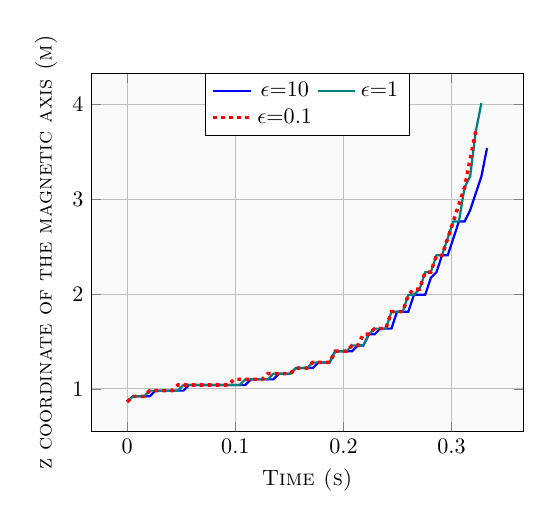
\begin{tikzpicture}[scale=0.8,>=latex]
\begin{axis}[xlabel=\textsc{{Time (s)}}, ylabel=\textsc{{z coordinate of the magnetic axis (m)}}, ymajorgrids, xmajorgrids, axis background/.style={fill=gray!4}, legend style={legend columns=2,at={(0.5,1.0)},anchor=north}]
\addplot+[color=blue,line width=1pt,mark=none] coordinates {(0, 0.86275)	(0.0052, 0.92225)	(0.0104, 0.92225)	(0.0156, 0.92225)	(0.0208, 0.92225)	(0.026, 0.98175)	(0.0312, 0.98175)	(0.0364, 0.98175)	(0.0416, 0.98175)	(0.0468, 0.98175)	(0.052, 0.98175)	(0.0572, 1.04125)	(0.0624, 1.04125)	(0.0676, 1.04125)	(0.0728, 1.04125)	(0.078, 1.04125)	(0.0832, 1.04125)	(0.0884, 1.04125)	(0.0936, 1.04125)	(0.0988, 1.04125)	(0.104, 1.04125)	(0.1092, 1.04125)	(0.1144, 1.10075)	(0.1196, 1.10075)	(0.1248, 1.10075)	(0.13, 1.10075)	         (0.1352, 1.10075)	(0.1404, 1.16025)	(0.1456, 1.16025)	(0.1508, 1.16025)	(0.156, 1.21975)	(0.1612, 1.21975)	(0.1664, 1.21975)	(0.1716, 1.21975)	(0.1768, 1.27925)	(0.182, 1.27925)	(0.1872, 1.27925)	(0.1924, 1.39825)	(0.1976, 1.39825)	(0.2028, 1.39825)	(0.208, 1.39825)	(0.2132, 1.45775)	(0.2184, 1.45775)	(0.2236, 1.57675)	(0.2288, 1.57675)    (0.234, 1.63625)	(0.2392, 1.63625)	(0.2444, 1.63625)      (0.2496, 1.81475)	(0.2548, 1.81475)	(0.26, 1.81475)	       (0.2652, 1.99325)	(0.2704, 1.99325)	(0.2756, 1.99325)      (0.2808, 2.17175)    (0.2860, 2.23125)      (0.2912, 2.40975)   (0.2964, 2.40975)   (0.3016, 2.58825)     (0.3068, 2.76675)     (0.3120, 2.76675)     (0.3172, 2.88575)      (0.3224, 3.06425)   (0.3276, 3.24275)   (0.3328, 3.54025)};
\addplot+[color=teal,line width=1pt,mark=none] coordinates {(0, 0.86275)	(0.0052, 0.92225)	(0.0104, 0.92225)	(0.0156, 0.92225)	(0.0208, 0.98175)	(0.026, 0.98175)	(0.0312, 0.98175)	(0.0364, 0.98175)	(0.0416, 0.98175)	(0.0468, 0.98175)	(0.052, 1.04125)	(0.0572, 1.04125)	(0.0624, 1.04125)	(0.0676, 1.04125)	(0.0728, 1.04125)	(0.078, 1.04125)	(0.0832, 1.04125)	(0.0884, 1.04125)	(0.0936, 1.04125)	(0.0988, 1.04125)	(0.104, 1.04125)	(0.1092, 1.10075)	(0.1144, 1.10075)	(0.1196, 1.10075)	(0.1248, 1.10075)	(0.13, 1.10075)	(0.1352, 1.16025)	(0.1404, 1.16025)	(0.1456, 1.16025)	(0.1508, 1.16025)	(0.156, 1.21975)	(0.1612, 1.21975)	(0.1664, 1.21975)	(0.1716, 1.27925)	(0.1768, 1.27925)	(0.182, 1.27925)	(0.1872, 1.27925)	(0.1924, 1.39825)	(0.1976, 1.39825)	(0.2028, 1.39825)	(0.208, 1.45775)	(0.2132, 1.45775)	(0.2184, 1.45775)	(0.2236, 1.57675)	(0.2288, 1.63625)   (0.234, 1.63625)	(0.2392, 1.63625)	(0.2444, 1.81475)	(0.2496, 1.81475)	(0.2548, 1.81475)	(0.26, 1.99325)   (0.2652, 1.99325)     (0.2704, 2.05275)     (0.2756, 2.23125)     (0.2808, 2.23125)     (0.286, 2.40975)      (0.2912, 2.40975)   (0.2964, 2.58825)     (0.3016, 2.76675)     (0.3068, 2.76675)     (0.3120, 3.12375)     (0.3172, 3.24275)    (0.3224, 3.71875)  (0.3276, 4.01625)};
%last two are already set
\addplot+[color=red,line width=1pt,mark=none,ultra thick,dotted] coordinates {(0, 0.86275)	(0.0052, 0.92225)	(0.0104, 0.92225)	(0.0156, 0.92225)	(0.0208, 0.98175)	(0.026, 0.98175)	(0.0312, 0.98175)	(0.0364, 0.98175)	(0.0416, 0.98175)	(0.0468, 1.04125)	(0.052, 1.04125)	(0.0572, 1.04125)	(0.0624, 1.04125)	(0.0676, 1.04125)	(0.0728, 1.04125)	(0.078, 1.04125)	(0.0832, 1.04125)	(0.0884, 1.04125)	(0.0936, 1.04125)	(0.0988, 1.10075)	(0.104, 1.10075)	(0.1092, 1.10075)	(0.1144, 1.10075)	(0.1196, 1.10075)	(0.1248, 1.10075)	(0.13, 1.16025)	(0.1352, 1.16025)	(0.1404, 1.16025)	(0.1456, 1.16025)	(0.1508, 1.16025)	(0.156, 1.21975)	(0.1612, 1.21975)	(0.1664, 1.21975)	(0.1716, 1.27925)	(0.1768, 1.27925)	(0.182, 1.27925)	(0.1872, 1.27925)	(0.1924, 1.39825)	(0.1976, 1.39825)	(0.2028, 1.39825)	(0.208, 1.45775)	(0.2132, 1.45775)	(0.2184, 1.57675)	(0.2236, 1.57675)	(0.2288, 1.63625)   (0.234, 1.63625)	(0.2392, 1.63625)	(0.2444, 1.81475)	(0.2496, 1.81475)	(0.2548, 1.81475)	(0.26, 1.99325)   (0.2652, 2.05275)     (0.2704, 2.05275)     (0.2756, 2.23125)     (0.2808, 2.23125)     (0.286, 2.40975)      (0.2912, 2.40975)   (0.2964, 2.58825)     (0.3016, 2.76675)     (0.3068, 2.94525)     (0.3120, 3.12375)     (0.3172, 3.42125)     (0.3224, 3.71875) };
\legend{$\epsilon$=10,$\epsilon$=1,$\epsilon$=0.1}
\end{axis}
\end{tikzpicture}
\caption{3 drag coefficients}
\label{fig:z_magneticaxis_15_15eV_time_eps+1-1}
\end{subfigure} 
\caption{Evolution of the z coordinate of the magnetic axis over time for different viscosity and drag coefficients.}
\label{fig:z_magneticaxis_15_15eV_time}
\end{figure}

\begin{figure}[!h]
\centering
\begin{subfigure}[b]{0.5\textwidth} 
\centering
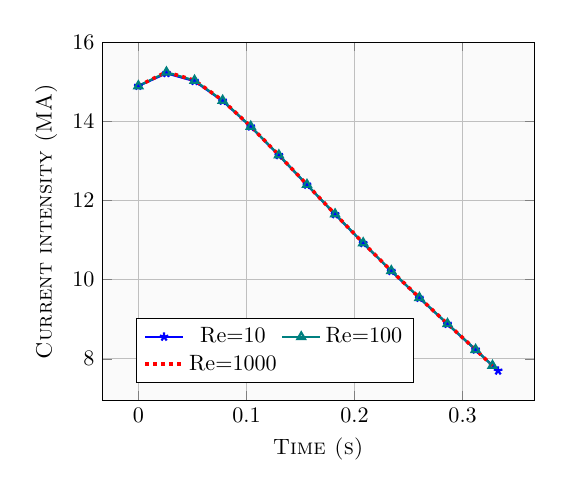
\begin{tikzpicture}[scale=0.8,>=latex]
\begin{axis}[scaled y ticks=base 10:-6, ytick scale label code/.code={}, xlabel=\textsc{{Time (s)}}, ylabel=\textsc{{Current intensity (MA)}}, ymajorgrids, xmajorgrids, axis background/.style={fill=gray!4}, legend style={legend columns=2,at={(0.4,0.05)},anchor=south}]
\addplot+[color=blue,line width=1pt,mark=star] coordinates {(0, 1.48934e+07) (0.026, 1.52149e+07) (0.052, 1.50161e+07) (0.078, 1.45168e+07) (0.104 , 1.38643e+07) (0.13, 1.31421e+07) (0.156, 1.23954e+07) (0.182, 1.16501e+07) (0.208, 1.09213e+07) (0.234, 1.02167e+07) (0.26, 9.53784e+06) (0.286, 8.87986e+06) (0.312, 8.22953e+06) (0.3328, 7.69845e+06)};
\addplot+[color=teal,line width=1pt,mark=triangle] coordinates {(0, 1.48934e+07) (0.026, 1.52405e+07) (0.052, 1.5032e+07) (0.078, 1.45262e+07) (0.104 , 1.38697e+07) (0.13, 1.31466e+07) (0.156, 1.24002e+07) (0.182, 1.16557e+07) (0.208, 1.09273e+07) (0.234, 1.02225e+07) (0.26, 9.54294e+06) (0.286, 8.88372e+06) (0.312, 8.23127e+06) (0.3276, 7.82844e+06)};
\addplot+[color=red,line width=1pt,mark=none,ultra thick,dotted] coordinates {(0, 1.48934e+07) (0.026, 1.52495e+07) (0.052, 1.50363e+07) (0.078, 1.45283e+07) (0.104 , 1.38704e+07) (0.13, 1.31472e+07) (0.156, 1.24011e+07) (0.182, 1.16571e+07) (0.208, 1.09291e+07) (0.234, 1.02241e+07) (0.26, 9.54422e+06) (0.286, 8.88477e+06) (0.312, 8.23172e+06) (0.3276, 7.82664e+06)};
\legend{Re=10,Re=100,Re=1000}
\end{axis}
\end{tikzpicture}
\caption{3 viscosity coefficients}
\label{fig:current_variousvisc_time}
\end{subfigure}%
~
\begin{subfigure}[b]{0.5\textwidth} 
\centering
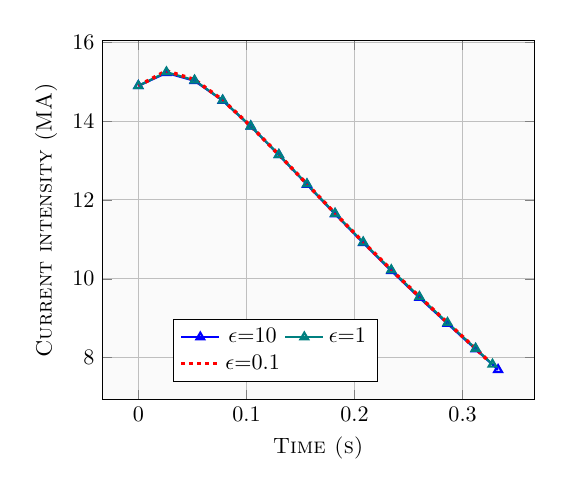
\begin{tikzpicture}[scale=0.8,>=latex]
\begin{axis}[scaled y ticks=base 10:-6, ytick scale label code/.code={}, xlabel=\textsc{{Time (s)}}, ylabel=\textsc{{Current intensity (MA)}}, ymajorgrids, xmajorgrids, axis background/.style={fill=gray!4}, legend style={legend columns=2,at={(0.4,0.05)},anchor=south}]
\addplot+[color=blue,line width=1pt,mark=triangle] coordinates {(0, 1.48934e+07) (0.026, 1.5222e+07) (0.052, 1.50214e+07) (0.078, 1.45207e+07) (0.104 , 1.38657e+07) (0.13, 1.3141e+07) (0.156, 1.23914e+07) (0.182, 1.16431e+07) (0.208, 1.09114e+07) (0.234, 1.0204e+07) (0.26, 9.52287e+06) (0.286, 8.86403e+06) (0.312, 8.21639e+06) (0.3328, 7.69489e+06)};
\addplot+[color=teal,line width=1pt,mark=triangle] coordinates {(0, 1.48934e+07) (0.026, 1.52405e+07) (0.052, 1.5032e+07) (0.078, 1.45262e+07) (0.104 , 1.38697e+07) (0.13, 1.31466e+07) (0.156, 1.24002e+07) (0.182, 1.16557e+07) (0.208, 1.09273e+07) (0.234, 1.02225e+07) (0.26, 9.54294e+06) (0.286, 8.88372e+06) (0.312, 8.23127e+06)  (0.3276, 7.82844e+06)};
\addplot+[color=red,line width=1pt,mark=none,ultra thick,dotted] coordinates {(0, 1.48934e+07) (0.026, 1.52739e+07) (0.052, 1.50496e+07) (0.078, 1.45334e+07) (0.104 , 1.38713e+07) (0.13, 1.31469e+07) (0.156, 1.24011e+07) (0.182, 1.16581e+07) (0.208, 1.09313e+07) (0.234, 1.02267e+07) (0.26, 9.5458e+06) (0.286, 8.88566e+06) (0.312, 8.22992e+06) (0.3224, 7.95837e+06)};
\legend{$\epsilon$=10,$\epsilon$=1,$\epsilon$=0.1}
\end{axis}
\end{tikzpicture}
\caption{3 drag coefficients}
\label{fig:current_variousdrag_time}
\end{subfigure}
\caption{Evolution of the current intensity inside the plasma chamber over time with different artificial viscosity and fictitious drag coefficients.}
\label{fig:current_time}
\end{figure}

We observe in Figures~\ref{fig:z_magneticaxis_15_15eV_time}
and~\ref{fig:current_time} that there is no significant change in the
curves for the current intensity and magnetic axis coordinate when we
vary the viscosity/drag coefficients, which could indicate
that the regularized model has already converged with such values and
there is no need to further decrease the regularization term as that
would induce more computational effort for the solver but with little
and insignificant impact on the relevant physical indicators or
properties.

% VDE happens at timestep 62 for drag coefficient epsilon = 0.1
% VDE happens at timestep 63 for drag coefficient epsilon = 1
% VDE happens at timestep 64 for drag coefficient epsilon = 10
% VDE happens at timestep 64 for drag coefficient Re = 10
% VDE happens at timestep 63 for drag coefficient Re = 100
% VDE happens at timestep 63 for drag coefficient Re = 1000

 A subtler effect of regularization, as explained in
Section~\ref{sec:regularization}, is that it sets a radial electric
field $\varphi(\psi),$ which is not constrained by the quasi-static
force-free model. This is thus an artificial radial electric field,
which interestingly enough, does not modify the magnetic field
evolution directly, since the curl of an electrostatic field vanishes
in the Faraday's law.  In Fig.~\ref{fig:EP_avg_psi_isovolumes}, we numerically compute
$\varphi(\psi)$ from $\Phi(R,Z)$ by performing an average of $\Phi$ along
the field lines which are contours of poloidal magnetic flux $\psi.$
This $\varphi(\Psi)$ is then plotted as a function of $\psi.$ Here we
shall classify two classes of magnetic field lines or constant $\psi$
surfaces (contour lines in the poloidal cross section of an
axisymmetric configuration).  Where $\psi$ forms closed contours in
the plasma domain, one has closed flux surfaces.  There are regions in
which $\psi$ contours or magnetic field lines intercept the chamber
wall, these are known as the open flux or magnetic field line region.
Since the chamber wall is a conductor and $\Phi$ is set to zero there,
so $\varphi$ on the open flux region is close to zero, in the order of
$10^{-10}$ to $10^{-8}$ (normalized unit) range.  The radial
electrostatic potential $\varphi(\psi)$ can take on a much larger value
inside the closed flux region, resulting in a sizable radial electric
field across the separatrix (if it exists) or the last closed flux
surface that scrapes off the chamber wall.

 By comparing Fig.~\ref{fig:EP_avg_psi_isovolumes_visc} and
Fig.~\ref{fig:EP_avg_psi_isovolumes_drag}, one can see that both the
fictitious drag $(\epsilon)$ and artificial viscosity $(\nu)$ produce
$\varphi(\psi)$ of comparable amplitude. In the case of artificial
viscosity, the $Re=100$ and $Re=1000$ cases appear to converge to the
same $\varphi(\psi).$ The fictitious drag coefficients of $\epsilon=10$
and $\epsilon=0.1$ evidently yield $\varphi(\psi)$ with sizable
difference in the closed flux region. 
That is also the case after 25 time steps in Figure~\ref{fig:EP_avg_psi_isovolumes_25dt}.
It should be emphasized again
that the $\varphi(\psi)$ so produced is an artificial radial electric
field, entirely the result of the regularization scheme. The
quasi-static MHD model itself does not physically constrain
$\varphi(\psi).$

 At a later time, all the fictitious drag and artificial viscosity coefficients produce almost identical $\varphi(\psi)$ amplitudes. This could be observed in  Figure~\ref{fig:EP_avg_psi_isovolumes_50dt} that shows the curves of electrostatic potential average in function of the poloidal magnetic flux function after 50 time steps, which corresponds to the time when the magnetic axis moves to mid-way (in vertical position) between the eventual impact point at the first wall and the initial state.
The same observation holds after 56 time steps in Figure~\ref{fig:EP_avg_psi_isovolumes_56dt}.

\pgfplotstableread{data_to_plot/dataRe10.txt}\tableone
\pgfplotstablecreatecol[create col/expr={-log10(-\thisrow{y} * 55000000)}]{log}\tableone
\pgfplotstablecreatecol[create col/expr={5*(\thisrow{x})}]{nonnormx}\tableone


\pgfplotstableread{data_to_plot/dataRe100.txt}\tabletwo
\pgfplotstablecreatecol[create col/expr={-log10(-\thisrow{y} * 55000000)}]{log}\tabletwo
\pgfplotstablecreatecol[create col/expr={5*(\thisrow{x})}]{nonnormx}\tabletwo


\pgfplotstableread{data_to_plot/dataRe1000.txt}\tablethree
\pgfplotstablecreatecol[create col/expr={-log10(-\thisrow{y} * 55000000)}]{log}\tablethree
\pgfplotstablecreatecol[create col/expr={5*(\thisrow{x})}]{nonnormx}\tablethree

\pgfplotstableread{data_to_plot/datadampV+1.txt}\tablefour
\pgfplotstablecreatecol[create col/expr={1/log10(-\thisrow{y})}]{log}\tablefour
\pgfplotstablecreatecol[create col/expr={5*(\thisrow{x})}]{nonnormx}\tablefour


\pgfplotstableread{data_to_plot/datadampV-1.txt}\tablesix
%\pgfplotstablecreatecol[create col/expr={-log10(-\thisrow{y}) * (\thisrow{y}<0) + log10(\thisrow{y}) * (\thisrow{y}>0)}]{log}\tablefive
\pgfplotstablecreatecol[create col/expr={\thisrow{y} > 0 ? -1/log10(\thisrow{y}) : 1/log10(-\thisrow{y})}]{log}\tablesix 
\pgfplotstablecreatecol[create col/expr={5*(\thisrow{x})}]{nonnormx}\tablesix

\pgfplotstableread{data_to_plot/datadampV0.txt}\tablefive
\pgfplotstablecreatecol[create col/expr={\thisrow{y} > 0 ? -1/log10(\thisrow{y}) : 1/log10(-\thisrow{y})}]{log}\tablefive 
\pgfplotstablecreatecol[create col/expr={5*(\thisrow{x})}]{nonnormx}\tablefive


\pgfplotstableread{data_to_plot/datadampV-2.txt}\tablesixbis
%\pgfplotstablecreatecol[create col/expr={-log10(-\thisrow{y}) * (\thisrow{y}<0) + log10(\thisrow{y}) * (\thisrow{y}>0)}]{log}\tablefive
\pgfplotstablecreatecol[create col/expr={\thisrow{y} > 0 ? -1/log10(\thisrow{y}) : 1/log10(-\thisrow{y})}]{log}\tablesixbis 
\pgfplotstablecreatecol[create col/expr={5*(\thisrow{x})}]{nonnormx}\tablesixbis

\begin{figure}[!h]
\centering
\begin{subfigure}[b]{0.47\textwidth} 
\begin{tikzpicture}[scale=0.80,>=latex]
\begin{axis}[xlabel=\textsc{{Poloidal magnetic flux function}}, ylabel=\textsc{{Electrostatic potential average}} , ytick={4,3,2,1,0,-1,-2}, yticklabels={$-10^{-4}$,$-10^{-3}$,$-10^{-2}$,$-10^{-1}$,$-1$,$-10$,$-100$}, ymajorgrids, xmajorgrids, axis background/.style={fill=gray!4}, legend style={legend columns=2,at={(0.66,1)},anchor=north}]
%\addplot+[color=blue,line width=1pt,mark=star] coordinates {(-8.29942, 1.48934e+07) (-7.16289, 1.52495e+07) (-6.01974, 1.50363e+07) (-4.87658, 1.45283e+07) (-3.73343 , 1.38704e+07) (-2.59028, 1.31472e+07) (-1.44713, 1.24011e+07) (-0.303973, 1.16571e+07) (0.83918, 1.09291e+07) (1.88233, 1.02241e+07) };
%\addplot+[color=teal,line width=1pt,mark=triangle] coordinates {(-8.29942, -1.8950599e-11) (-7.16289, -8.2132436e-11) (-6.01974, -2.3033332e-10) (-4.87658, -1.20993374e-9) (-3.73343 , -2.21793749e-9) (-2.59028, -1.93624069e-8) (-1.44713, -0.00000407647) (-0.303973, -0.00000387466) (0.83918, -0.00000304414) (1.88233, -8.08733057e-7)};
%\addplot+[color=red,line width=1pt,mark=none,ultra thick,dotted] coordinates {(-8.29942, -1.4556861e-11) (-7.16289, -6.4457328e-11) (-6.01974, -2.0733733e-10) (-4.87658, -1.16348118e-9) (-3.73343 , -2.13538999e-9) (-2.59028, -1.69946902e-8) (-1.44713, -0.00000468606) (-0.303973, -0.00000393359) (0.83918, -0.00000300482) (1.88233, -8.46751698e-7)};
\addplot+[color=blue,line width=1pt,mark=star] table[x=nonnormx, y=log] \tableone;
\addplot+[color=teal,line width=1pt,mark=triangle] table[x=nonnormx, y=log] \tabletwo;
\addplot+[color=red,line width=1pt,mark=o] table[x=nonnormx, y=log] \tablethree;
\legend{Re=10,Re=100,Re=1000}
\end{axis}
\end{tikzpicture}
\caption{3 viscosity coefficients}
\label{fig:EP_avg_psi_isovolumes_visc}
\end{subfigure}%
~
\begin{subfigure}[b]{0.47\textwidth} 
\centering
\begin{tikzpicture}[scale=0.80,>=latex]
\begin{axis}[xlabel=\textsc{{Poloidal magnetic flux function}}, ylabel=\textsc{{Electrostatic potential average}} , ytick={-0.0833,-0.125,-0.1666,-0.25,0,0.1666,0.25}, yticklabels={$-10^{-4.26}$,$-10^{0.26}$,$-10^{1.74}$,$-10^{3.74}$,0,$10^{1.74}$,$10^{3.74}$}, ymajorgrids, xmajorgrids, axis background/.style={fill=gray!4}, legend style={legend columns=2,at={(0.5,1)},anchor=north}]
%ytick={-0.0833,-0.125,-0.1666,-0.25,0,0.1666,0.25}, yticklabels={$-10^{-12}$,$-10^{-8}$,$-10^{-6}$,$-10^{-4}$,0,$10^{-6}$,$10^{-4}$}, ymajorgrids, xmajorgrids, axis background/.style={fill=gray!4}, legend style={legend columns=2,at={(0.5,1)},anchor=north}]
%ytick={-0.1515,-0.227,-0.303,-0.4545,0,0.303,0.4545}, yticklabels={$-10^{-4}$,$-1$,$-10^{2}$,$-10^{4}$,$1$,$10^{2}$,$10^{4}$},
\addplot+[color=blue,line width=1pt,mark=star] table[x=nonnormx, y=log] \tablefour;
\addplot+[color=teal,line width=1pt,mark=triangle] table[x=nonnormx, y=log] \tablefive;
\addplot+[color=red,line width=1pt,mark=o] table[x=nonnormx, y=log] \tablesix;
\addplot+[color=black,line width=1pt,mark=none] table[x=nonnormx, y=log] \tablesixbis;
\legend{$\epsilon$=10,$\epsilon$=1,$\epsilon$=0.1,$\epsilon$=0.01}
\end{axis}
\end{tikzpicture}
\caption{4 drag coefficients}
\label{fig:EP_avg_psi_isovolumes_drag}
\end{subfigure}
\caption{Evolution of the electrostatic potential average over poloidal magnetic flux function with different artificial viscosity and fictitious drag coefficients at the first time step.}
\label{fig:EP_avg_psi_isovolumes}
\end{figure}


%Add electrostatic potential average plots at t = 25 dt, i.e. t = 0.13

\pgfplotstableread{data_to_plot/datadampV+1_25dt.txt}\tablethirteen
\pgfplotstablecreatecol[create col/expr={\thisrow{y} > 0 ? -1/log10(\thisrow{y}) : 1/log10(-\thisrow{y})}]{log}\tablethirteen
\pgfplotstablecreatecol[create col/expr={5*(\thisrow{x})}]{nonnormx}\tablethirteen


\pgfplotstableread{data_to_plot/datadampV0_25dt.txt}\tablefourteen
\pgfplotstablecreatecol[create col/expr={\thisrow{y} > 0 ? -1/log10(\thisrow{y}) : 1/log10(-\thisrow{y})}]{log}\tablefourteen
\pgfplotstablecreatecol[create col/expr={5*(\thisrow{x})}]{nonnormx}\tablefourteen


\pgfplotstableread{data_to_plot/datadampV-1_25dt.txt}\tablefifteen
\pgfplotstablecreatecol[create col/expr={\thisrow{y} > 0 ? -1/log10(\thisrow{y}) : 1/log10(-\thisrow{y})}]{log}\tablefifteen
\pgfplotstablecreatecol[create col/expr={5*(\thisrow{x})}]{nonnormx}\tablefifteen


\pgfplotstableread{data_to_plot/dataRe10_25dt.txt}\tablesixteen
\pgfplotstablecreatecol[create col/expr={\thisrow{y} > 0 ? -1/log10(\thisrow{y}) : 1/log10(-\thisrow{y})}]{log}\tablesixteen
\pgfplotstablecreatecol[create col/expr={5*(\thisrow{x})}]{nonnormx}\tablesixteen


\pgfplotstableread{data_to_plot/dataRe100_25dt.txt}\tableseventeen
\pgfplotstablecreatecol[create col/expr={\thisrow{y} > 0 ? -1/log10(\thisrow{y}) : 1/log10(-\thisrow{y})}]{log}\tableseventeen
\pgfplotstablecreatecol[create col/expr={5*(\thisrow{x})}]{nonnormx}\tableseventeen


\pgfplotstableread{data_to_plot/dataRe1000_25dt.txt}\tableeighteen
\pgfplotstablecreatecol[create col/expr={\thisrow{y} > 0 ? -1/log10(\thisrow{y}) : 1/log10(-\thisrow{y})}]{log}\tableeighteen
\pgfplotstablecreatecol[create col/expr={5*(\thisrow{x})}]{nonnormx}\tableeighteen


\begin{figure}[!h]
\centering
\begin{subfigure}[b]{0.47\textwidth} 
\begin{tikzpicture}[scale=0.80,>=latex]
\begin{axis}[xlabel=\textsc{{Poloidal magnetic flux function}}, ylabel=\textsc{{Electrostatic potential average}} , ytick={-0.17420500732,-0.14835996906,-0.12919291255,-0.10266,0, 0.14835996906,0.17420500732}, yticklabels={-100,-10,-1,$-10^{-2}$,0,10,100}, ymajorgrids, xmajorgrids, axis background/.style={fill=gray!4}, legend style={legend columns=2,at={(0.4,1)},anchor=north}]
\addplot+[color=blue,line width=1pt,mark=star] table[x=nonnormx, y=log] \tablesixteen;
\addplot+[color=teal,line width=1pt,mark=triangle] table[x=nonnormx, y=log] \tableseventeen;
\addplot+[color=red,line width=1pt,mark=o] table[x=nonnormx, y=log] \tableeighteen;
\legend{Re=10,Re=100,Re=1000}
\end{axis}
\end{tikzpicture}
\caption{3 viscosity coefficients}
\label{fig:EP_avg_psi_isovolumes_visc_25dt}
\end{subfigure}%
~
\begin{subfigure}[b]{0.47\textwidth} 
\centering
\begin{tikzpicture}[scale=0.80,>=latex]
\begin{axis}[xlabel=\textsc{{Poloidal magnetic flux function}}, ylabel=\textsc{{Electrostatic potential average}} , ytick={-0.17420500732,-0.14835996906,-0.12919291255,-0.10266,0, 0.14835996906,0.17420500732}, yticklabels={-100,-10,-1,$-10^{-2}$,0,10,100}, ymajorgrids, xmajorgrids, axis background/.style={fill=gray!4}, legend style={legend columns=2,at={(0.4,1)},anchor=north}]
% ytick={-0.1666,-0.13768,-0.10266,0,0.1687}, yticklabels={-55,-3,$-10^{-2}$,0,65},
% ytick={-0.1666,-0.14836,-0.13768,-0.10266,0,0.1687}, yticklabels={-55,-10,-3,$-10^{-2}$,0,65}
\addplot+[color=blue,line width=1pt,mark=star] table[x=nonnormx, y=log] \tablethirteen;
\addplot+[color=teal,line width=1pt,mark=triangle] table[x=nonnormx, y=log] \tablefourteen;
\addplot+[color=red,line width=1pt,mark=o] table[x=nonnormx, y=log] \tablefifteen;
\legend{$\epsilon$=10,$\epsilon$=1,$\epsilon$=0.1}
\end{axis}
\end{tikzpicture}
\caption{3 drag coefficients}
\label{fig:EP_avg_psi_isovolumes_drag_25dt}
\end{subfigure}
\caption{Evolution of the electrostatic potential average over poloidal magnetic flux function with different artificial viscosity and fictitious drag coefficients after 25 time steps.}
\label{fig:EP_avg_psi_isovolumes_25dt}
\end{figure}


%Add electrostatic potential average plots at t = 50 dt, i.e. t = 0.26

\pgfplotstableread{data_to_plot/datadampV+1_50dt.txt}\tableten
\pgfplotstablecreatecol[create col/expr={-log10(-\thisrow{y} * 55000000)}]{log}\tableten
\pgfplotstablecreatecol[create col/expr={5*(\thisrow{x})}]{nonnormx}\tableten


\pgfplotstableread{data_to_plot/datadampV0_50dt.txt}\tableeleven
\pgfplotstablecreatecol[create col/expr={-log10(-\thisrow{y} * 55000000)}]{log}\tableeleven
\pgfplotstablecreatecol[create col/expr={5*(\thisrow{x})}]{nonnormx}\tableeleven


\pgfplotstableread{data_to_plot/datadampV-1_50dt.txt}\tabletwelve
\pgfplotstablecreatecol[create col/expr={-log10(-\thisrow{y} * 55000000)}]{log}\tabletwelve
\pgfplotstablecreatecol[create col/expr={5*(\thisrow{x})}]{nonnormx}\tabletwelve


\pgfplotstableread{data_to_plot/dataRe10_50dt.txt}\tableseven
\pgfplotstablecreatecol[create col/expr={-log10(-\thisrow{y} * 55000000)}]{log}\tableseven
\pgfplotstablecreatecol[create col/expr={5*(\thisrow{x})}]{nonnormx}\tableseven


\pgfplotstableread{data_to_plot/dataRe100_50dt.txt}\tableeight
\pgfplotstablecreatecol[create col/expr={-log10(-\thisrow{y} * 55000000)}]{log}\tableeight
\pgfplotstablecreatecol[create col/expr={5*(\thisrow{x})}]{nonnormx}\tableeight


\pgfplotstableread{data_to_plot/dataRe1000_50dt.txt}\tablenine
\pgfplotstablecreatecol[create col/expr={-log10(-\thisrow{y} * 55000000)}]{log}\tablenine
\pgfplotstablecreatecol[create col/expr={5*(\thisrow{x})}]{nonnormx}\tablenine


\begin{figure}[!h]
\centering
\begin{subfigure}[b]{0.47\textwidth} 
\begin{tikzpicture}[scale=0.80,>=latex]
\begin{axis}[xlabel=\textsc{{Poloidal magnetic flux function}}, ylabel=\textsc{{Electrostatic potential average}} , ytick={4,3,2,1,0,-1,-2}, yticklabels={$-10^{-4}$,$-10^{-3}$,$-10^{-2}$,$-10^{-1}$,$-1$,$-10$,$-100$}, ymajorgrids, xmajorgrids, axis background/.style={fill=gray!4}, legend style={legend columns=2,at={(0.66,1)},anchor=north}]
\addplot+[color=blue,line width=1pt,mark=star] table[x=nonnormx, y=log] \tableseven;
\addplot+[color=teal,line width=1pt,mark=triangle] table[x=nonnormx, y=log] \tableeight;
\addplot+[color=red,line width=1pt,mark=o] table[x=nonnormx, y=log] \tablenine;
\legend{Re=10,Re=100,Re=1000}
\end{axis}
\end{tikzpicture}
\caption{3 viscosity coefficients}
\label{fig:EP_avg_psi_isovolumes_visc_50dt}
\end{subfigure}%
~
\begin{subfigure}[b]{0.47\textwidth} 
\centering
\begin{tikzpicture}[scale=0.80,>=latex]
\begin{axis}[xlabel=\textsc{{Poloidal magnetic flux function}}, ylabel=\textsc{{Electrostatic potential average}} , ytick={4,3,2,1,0,-1,-2}, yticklabels={$-10^{-4}$,$-10^{-3}$,$-10^{-2}$,$-10^{-1}$,$-1$,$-10$,$-100$}, ymajorgrids, xmajorgrids, axis background/.style={fill=gray!4}, legend style={legend columns=2,at={(0.6,1)},anchor=north}]
\addplot+[color=blue,line width=1pt,mark=star] table[x=nonnormx, y=log] \tableten;
\addplot+[color=teal,line width=1pt,mark=triangle] table[x=nonnormx, y=log] \tableeleven;
\addplot+[color=red,line width=1pt,mark=o] table[x=nonnormx, y=log] \tabletwelve;
\legend{$\epsilon$=10,$\epsilon$=1,$\epsilon$=0.1}
\end{axis}
\end{tikzpicture}
\caption{3 drag coefficients}
\label{fig:EP_avg_psi_isovolumes_drag_50dt}
\end{subfigure}
\caption{Evolution of the electrostatic potential average over poloidal magnetic flux function with different artificial viscosity and fictitious drag coefficients after 50 time steps.}
\label{fig:EP_avg_psi_isovolumes_50dt}
\end{figure}


%Add electrostatic potential average plots at t = 56 dt, i.e. t = 0.2912

\pgfplotstableread{data_to_plot/datadampV+1_56dt.txt}\tablenineteen
\pgfplotstablecreatecol[create col/expr={-log10(-\thisrow{y} * 55000000)}]{log}\tablenineteen
\pgfplotstablecreatecol[create col/expr={5*(\thisrow{x})}]{nonnormx}\tablenineteen


\pgfplotstableread{data_to_plot/datadampV0_56dt.txt}\tabletwenty
\pgfplotstablecreatecol[create col/expr={-log10(-\thisrow{y} * 55000000)}]{log}\tabletwenty
\pgfplotstablecreatecol[create col/expr={5*(\thisrow{x})}]{nonnormx}\tabletwenty


\pgfplotstableread{data_to_plot/datadampV-1_56dt.txt}\tabletwentyone
\pgfplotstablecreatecol[create col/expr={-log10(-\thisrow{y} * 55000000)}]{log}\tabletwentyone
\pgfplotstablecreatecol[create col/expr={5*(\thisrow{x})}]{nonnormx}\tabletwentyone


\pgfplotstableread{data_to_plot/dataRe10_56dt.txt}\tabletwentytwo
\pgfplotstablecreatecol[create col/expr={-log10(-\thisrow{y} * 55000000)}]{log}\tabletwentytwo
\pgfplotstablecreatecol[create col/expr={5*(\thisrow{x})}]{nonnormx}\tabletwentytwo


\pgfplotstableread{data_to_plot/dataRe100_56dt.txt}\tabletwentythree
\pgfplotstablecreatecol[create col/expr={-log10(-\thisrow{y} * 55000000)}]{log}\tabletwentythree
\pgfplotstablecreatecol[create col/expr={5*(\thisrow{x})}]{nonnormx}\tabletwentythree


\pgfplotstableread{data_to_plot/dataRe1000_56dt.txt}\tabletwentyfour
\pgfplotstablecreatecol[create col/expr={-log10(-\thisrow{y} * 55000000)}]{log}\tabletwentyfour
\pgfplotstablecreatecol[create col/expr={5*(\thisrow{x})}]{nonnormx}\tabletwentyfour


\begin{figure}[!h]
\centering
\begin{subfigure}[b]{0.47\textwidth} 
\begin{tikzpicture}[scale=0.80,>=latex]
\begin{axis}[xlabel=\textsc{{Poloidal magnetic flux function}}, ylabel=\textsc{{Electrostatic potential average}} , ytick={4,3,2,1,0,-1,-2}, yticklabels={$-10^{-4}$,$-10^{-3}$,$-10^{-2}$,$-10^{-1}$,$-1$,$-10$,$-100$}, ymajorgrids, xmajorgrids, axis background/.style={fill=gray!4}, legend style={legend columns=2,at={(0.66,1)},anchor=north}]
\addplot+[color=blue,line width=1pt,mark=star] table[x=nonnormx, y=log] \tabletwentytwo;
\addplot+[color=teal,line width=1pt,mark=triangle] table[x=nonnormx, y=log] \tabletwentythree;
\addplot+[color=red,line width=1pt,mark=o] table[x=nonnormx, y=log] \tabletwentyfour;
\legend{Re=10,Re=100,Re=1000}
\end{axis}
\end{tikzpicture}
\caption{3 viscosity coefficients}
\label{fig:EP_avg_psi_isovolumes_visc_56dt}
\end{subfigure}%
~
\begin{subfigure}[b]{0.47\textwidth} 
\centering
\begin{tikzpicture}[scale=0.80,>=latex]
\begin{axis}[xlabel=\textsc{{Poloidal magnetic flux function}}, ylabel=\textsc{{Electrostatic potential average}} , ytick={4,3,2,1,0,-1,-2}, yticklabels={$-10^{-4}$,$-10^{-3}$,$-10^{-2}$,$-10^{-1}$,$-1$,$-10$,$-100$}, ymajorgrids, xmajorgrids, axis background/.style={fill=gray!4}, legend style={legend columns=2,at={(0.6,1)},anchor=north}]
\addplot+[color=blue,line width=1pt,mark=star] table[x=nonnormx, y=log] \tablenineteen;
\addplot+[color=teal,line width=1pt,mark=triangle] table[x=nonnormx, y=log] \tabletwenty;
\addplot+[color=red,line width=1pt,mark=o] table[x=nonnormx, y=log] \tabletwentyone;
\legend{$\epsilon$=10,$\epsilon$=1,$\epsilon$=0.1}
\end{axis}
\end{tikzpicture}
\caption{3 drag coefficients}
\label{fig:EP_avg_psi_isovolumes_drag_56dt}
\end{subfigure}
\caption{Evolution of the electrostatic potential average over poloidal magnetic flux function with different artificial viscosity and fictitious drag coefficients after 56 time steps.}
\label{fig:EP_avg_psi_isovolumes_56dt}
\end{figure}


\begin{figure}[!h]
\centering
\begin{subfigure}[b]{0.32\textwidth} 
\begin{center}
\includegraphics[width=\textwidth]{psi_Re10.png}
\caption{${\mathrm Re}=10$}
\label{fig:psi_drag_10}
\end{center}
\end{subfigure}%
~
\begin{subfigure}[b]{0.32\textwidth} 
\begin{center}
\includegraphics[width=\textwidth]{psi_Re100.png}
\caption{${\mathrm Re}=100$}
\label{fig:psi_drag_100}
\end{center}
\end{subfigure}%
~
\begin{subfigure}[b]{0.32\textwidth} 
\begin{center}
\includegraphics[width=\textwidth]{psi_Re1000.png}
\caption{${\mathrm Re}=1000$}
\label{fig:psi_drag_1000}
\end{center}
\end{subfigure}
\caption{The poloidal magnetic flux function with different artificial viscosity coefficients at the first time step}
\label{fig:psi_1st_step}
\end{figure}

\begin{figure}[!h]
\centering
\begin{subfigure}[b]{0.32\textwidth} 
\begin{center}
\includegraphics[width=\textwidth]{Deltapsi_10-1000.png}
\caption{$\Psi({\mathrm Re}=10) - \Psi({\mathrm Re}=1000)$}
\label{fig:Deltapsi_drag_10}
\end{center}
\end{subfigure}%
~
\begin{subfigure}[b]{0.32\textwidth} 
\begin{center}
\includegraphics[width=\textwidth]{Deltapsi_100-1000.png}
\caption{$\Psi({\mathrm Re}=100) - \Psi({\mathrm Re}=1000)$}
\label{fig:Deltapsi_drag_100}
\end{center}
\end{subfigure}%
~
\begin{subfigure}[b]{0.32\textwidth} 
\begin{center}
\includegraphics[width=\textwidth]{psi_Re1000.png}
\caption{$\Psi({\mathrm Re}=1000)$}
\label{fig:psi_drag_1000_bis}
\end{center}
\end{subfigure}
\caption{The poloidal magnetic flux function for ${\mathrm Re} = 1000$ and the differences $\Psi({\mathrm Re}=100) - \Psi({\mathrm Re}=1000)$ and $\Psi({\mathrm Re}=10) - \Psi({\mathrm Re}=1000)$ at the first time step.}
\label{fig:deltapsi_1st_step}
\end{figure}

\begin{figure}[!h]
\centering
\begin{subfigure}[b]{0.32\textwidth} 
\begin{center}
\includegraphics[width=\textwidth]{Deltapsi_10-1000_t50.png}
\caption{$\Psi({\mathrm Re}=10) - \Psi({\mathrm Re}=1000)$}
\label{fig:Deltapsi_drag_10_t50}
\end{center}
\end{subfigure}%
~
\begin{subfigure}[b]{0.32\textwidth} 
\begin{center}
\includegraphics[width=\textwidth]{Deltapsi_100-1000_t50.png}
\caption{$\Psi({\mathrm Re}=100) - \Psi({\mathrm Re}=1000)$}
\label{fig:Deltapsi_drag_100_t50}
\end{center}
\end{subfigure}%
~
\begin{subfigure}[b]{0.32\textwidth} 
\begin{center}
\includegraphics[width=\textwidth]{psi_Re1000_t50.png}
\caption{$\Psi({\mathrm Re}=1000)$}
\label{fig:psi_drag_1000_t50}
\end{center}
\end{subfigure}
\caption{The poloidal magnetic flux function for ${\mathrm Re} = 1000$ and the differences $\Psi({\mathrm Re}=100) - \Psi({\mathrm Re}=1000)$ and $\Psi({\mathrm Re}=10) - \Psi({\mathrm Re}=1000)$ after 50 time steps.}
\label{fig:deltapsi_50th_step}
\end{figure}

\begin{figure}[!h]
\centering
\begin{subfigure}[b]{0.32\textwidth} 
\begin{center}
\includegraphics[width=\textwidth]{EP_Re10.png}
\caption{${\mathrm Re}=10$}
\label{fig:EP_drag_10}
\end{center}
\end{subfigure}%
~
\begin{subfigure}[b]{0.32\textwidth} 
\begin{center}
\includegraphics[width=\textwidth]{EP_Re100.png}
\caption{${\mathrm Re}=100$}
\label{fig:EP_drag_100}
\end{center}
\end{subfigure}%
~
\begin{subfigure}[b]{0.32\textwidth} 
\begin{center}
\includegraphics[width=\textwidth]{EP_Re1000.png}
\caption{${\mathrm Re}=1000$}
\label{fig:EP_drag_1000}
\end{center}
\end{subfigure}
\caption{The electrostatic potential with different artificial viscosity coefficients at the first time step.}
\label{fig:EP_1st_step}
\end{figure}
\begin{figure}[!h]
\centering
\begin{subfigure}[b]{0.32\textwidth} 
\begin{center}
\includegraphics[width=\textwidth]{DeltaEP_10-1000.png}
\caption{$\Phi({\mathrm Re}=10) - \Phi({\mathrm Re}=1000)$}
\label{fig:DeltaEP_drag_10}
\end{center}
\end{subfigure}%
~
\begin{subfigure}[b]{0.32\textwidth} 
\begin{center}
\includegraphics[width=\textwidth]{DeltaEP_100-1000.png}
\caption{$\Phi({\mathrm Re}=100) - \Phi({\mathrm Re}=1000)$}
\label{fig:DeltaEP_drag_100}
\end{center}
\end{subfigure}%
~
\begin{subfigure}[b]{0.32\textwidth} 
\begin{center}
\includegraphics[width=\textwidth]{EP_Re1000.png}
\caption{$\Phi({\mathrm Re}=1000)$}
\label{fig:EP_drag_1000_bis}
\end{center}
\end{subfigure}
\caption{The electrostatic potential for ${\mathrm Re} = 1000$ and the differences $\Phi({\mathrm Re}=100) - \Phi({\mathrm Re}=1000)$ and $\Phi({\mathrm Re}=10) - \Phi({\mathrm Re}=1000)$ at the first time step.}
\label{fig:DeltaEP_1st_step}
\end{figure}

 Figures~\ref{fig:psi_1st_step}--\ref{fig:deltapsi_50th_step} and~\ref{fig:EP_1st_step}--\ref{fig:DeltaEP_50th_step} show the poloidal magnetic flux function and the electrostatic potential respectively with different artificial viscosity coefficients at the first time step and after 50 time steps. The former figures show that the poloidal magnetic flux function is identical for the three viscosity coefficients whereas the latter figures show that there are differences in the electrostatic potential but these tend to be rather minimal. 

\begin{figure}[!h]
\centering
\begin{subfigure}[b]{0.32\textwidth} 
\begin{center}
\includegraphics[width=\textwidth]{EP_Re10_t50.png}
\caption{${\mathrm Re}=10$}
\label{fig:EP_drag_10_t50}
\end{center}
\end{subfigure}%
~
\begin{subfigure}[b]{0.32\textwidth} 
\begin{center}
\includegraphics[width=\textwidth]{EP_Re100_t50.png}
\caption{${\mathrm Re}=100$}
\label{fig:EP_drag_100_t50}
\end{center}
\end{subfigure}%
~
\begin{subfigure}[b]{0.32\textwidth} 
\begin{center}
\includegraphics[width=\textwidth]{EP_Re1000_t50.png}
\caption{${\mathrm Re}=1000$}
\label{fig:EP_drag_1000_t50}
\end{center}
\end{subfigure}
\caption{The electrostatic potential with different artificial viscosity coefficients after 50 time steps.}
\label{fig:EP_50th_step}
\end{figure}

\begin{figure}[!h]
\centering
\begin{subfigure}[b]{0.32\textwidth} 
\begin{center}
\includegraphics[width=\textwidth]{DeltaEP_10-1000_t50.png}
\caption{$\Phi({\mathrm Re}=10) - \Phi({\mathrm Re}=1000)$}
\label{fig:DeltaEP_drag_10_t50}
\end{center}
\end{subfigure}%
~
\begin{subfigure}[b]{0.32\textwidth} 
\begin{center}
\includegraphics[width=\textwidth]{DeltaEP_100-1000_t50.png}
\caption{$\Phi({\mathrm Re}=100) - \Phi({\mathrm Re}=1000)$}
\label{fig:DeltaEP_drag_100_t50}
\end{center}
\end{subfigure}%
~
\begin{subfigure}[b]{0.32\textwidth} 
\begin{center}
\includegraphics[width=\textwidth]{EP_Re1000_t50.png}
\caption{$\Phi({\mathrm Re}=1000)$}
\label{fig:EP_drag_1000_t50_bis}
\end{center}
\end{subfigure}
\caption{The electrostatic potential for ${\mathrm Re} = 1000$ and the differences $\Phi({\mathrm Re}=100) - \Phi({\mathrm Re}=1000)$ and $\Phi({\mathrm Re}=10) - \Phi({\mathrm Re}=1000)$ after 50 time steps.}
\label{fig:DeltaEP_50th_step}
\end{figure}

